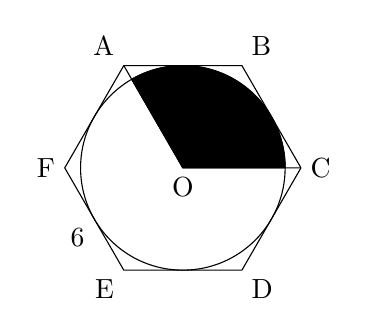
\begin{tikzpicture}
\draw(0,0)node[anchor=north]{O}+(1.5,0)node[anchor=west]{C}--(60:1.5)node[anchor=south west]{B}--(120:1.5)node[anchor=south east]{A}--(180:1.5)node[anchor=east]{F}--(240:1.5)node[anchor=north
east]{E}--(300:1.5)node[anchor=north west]{D}--(360:1.5);
\draw(120:1.5)--(0,0)--(1.5,0);
\draw(0,0)circle(1.2990381056766579701455847561294);
\filldraw(0,0)--(1.2990381056766579701455847561294,0)arc(0:120:1.2990381056766579701455847561294)--cycle;
\draw(210:1.2990381056766579701455847561294)node[anchor=north east]{6};
\end{tikzpicture}
Circle O is inscribed inside regular hexagon $ABCDEF$. $EF = 6$. What is the area of the sector of circle O inside rhombus OABC?


\ifsat
	\begin{enumerate}[label=\Alph*)]
		\item  $2\pi$
		\item  $6 \pi$
		\item  $9\pi$%
		\item  $27\pi$
	\end{enumerate}
\else
\fi

\ifacteven
	\begin{enumerate}[label=\textbf{\Alph*.},itemsep=\fill,align=left]
		\setcounter{enumii}{5}
		\item  $2\pi$
		\item  $6 \pi$
		\item  $9\pi$%
		\addtocounter{enumii}{1}
		\item  $12\pi$
		\item  $27\pi$
	\end{enumerate}
\else
\fi

\ifactodd
	\begin{enumerate}[label=\textbf{\Alph*.},itemsep=\fill,align=left]
		\item  $2\pi$
		\item  $6 \pi$
		\item  $9\pi$%
		\item  $12\pi$
		\item  $27\pi$
	\end{enumerate}
\else
\fi

\ifgridin
  $9\pi$%
		
\else
\fi

